\section{Experiments}
\label{sec:experiments}


\subsection{Image datasets}
\label{sec:dataset}
We use image-caption datasets for our experiments.
F8k \citep{rashtchian2010collecting} consists of 8000 images and five
captions for each image. F30k \citep{young2014image} extends the F8k and contains 31,783 images
with five captions each summing up to 158,915 sentences. For both data
sets we use the splits from \cite{karpathy2014deep}, leaving out 1000
images for validation and 1000 for testing from each
set. Table~\ref{tab:flickr} summarizes the statistics of the Flickr
image-caption datasets.



\begin{table}[h]
\centering
\begin{tabular}{l|r|r}
                    & F8k    & F30k   \\ \hline
Train images        & 6,000       & 29,780  \\
Validation images   & 1,000       & 1,000   \\
Test images         & 1,000       & 1,000   \\
Image in total      & 8,000       & 31,780  \\
Captions per image  & 5           & 5      \\
Captions in total   & 40,000      & 158,900 \\
\end{tabular}
\caption{\textit{Flickr image caption datasets.}}
\label{tab:flickr}
\end{table}
For the Single-concept image descriptions experiments reported in
section \ref{sec:experiments-production}, we also use the ILSVRC2012
subset of ImageNet \citep{russakovsky2015imagenet}, a widely-used data set in the computer vision
community. It is an image database that annotates the WordNet noun
synset hierarchy with images. It contains 500 images per synset on
average.

\subsection{Word similarity experiments}
\label{sec:experiments-wsj}
A common evaluation task for assessing the quality of learned semantic
vectors for words is measuring word similarity. A number of
experiments have elicited human ratings on the similarity and/or
relatedness of a list of word pairs. For instance one of the data sets
we used was the SimLex999 data set, which contains similarity judgments
for 666 noun pairs (organ-liver 6.15), 222 verb pairs (occur-happen 1.38)
and \mbox{111 adjective pairs} (nice-cruel 0.67) elicited by 500 participants
recruited from \mbox{Mechanical Turk}\label{rev:similarity_example}.
These types of data sets are commonly used as
benchmarks for models of distributional semantics, where the learned
representations are expected to show a significant positive
correlation with human similarity judgments on a large number of word
pairs.


We selected a subset of the existing benchmarks according to the size
of their word pairs that overlap with our restricted vocabulary. We
ran a statistical power analysis test to estimate the minimum number
of required word pairs needed in our experiments. The projected sample
size was $N=210$ with $p=.05$, effect-size $r=.2$ and
$\mathit{power}=0.9$.  Thus some of the well-known benchmarks were
excluded due to their small sample size after we excluded words not
present in our datasets.\footnote{These include RG-65
  \citep{rubenstein1965contextual}, MC-30 \citep{miller1991contextual}
  and YP-130 \citep{yang2006verb}.}


The four standard benchmarks that contain the minimum number of word
pairs are: the full WS-353 \citep{finkelstein2001placing}, MTurk-771
\citep{radinsky2011word}, MEN \citep{bruni2014multimodal} and
SimLex999 \citep{hill2015simlex}. Note that the MTurk dataset only
contains similarity judgments for nouns. Also, a portion of the full
WordSim-353 dataset reports relatedness ratings instead of word
similarity.

\subsection{Effect of concreteness on similarity judgments}
\label{sec:effect-concrete}
The word similarity judgments provide a macro evaluation about the
overall quality of the learned word representations. For more
fine-grained analysis we turn to the dichotomy of concrete (e.g.\ {\it
  chair, car}) versus abstract (e.g.\ {\it love, sorrow}) nouns.
Evidence presented by \cite{recchia2012semantic} shows that in naming
and lexical decision tasks the early activation of abstract concepts
is facilitated by rich linguistic contexts, while physical contexts
promote the activation of concrete concepts. Based on these recent
findings, \cite{bruni2014multimodal} suggest that in case of
computational models {\it concrete} words (such as names for physical
objects and visual properties) are easier to learn from
perceptual/visual input and {\it abstract} words are mainly learned
based on their co-occurrence with other words in text.  Following
\cite{bruni2014multimodal}, but using novel methodology, we also test
this idea and examine whether more concrete words benefit more from
visual features compared with less concrete ones.

In their work \cite{bruni2014multimodal} use the automatic method from \cite{turney2011literal}
to assign concreteness values to words and split the MEN corpus in
concrete and abstract chunks. From their experiments they draw the
conclusion that visual information boosts their models' performance on
concrete nouns. However, whereas the multi-modal embeddings of
\cite{bruni2014multimodal} are trained using an unbalanced corpus of
large quantities of textual information and far poorer visual stimuli,
our visual embeddings are learned on a parallel corpus of sentences
paired with images. To our purposes, this balance in the sources of
information is critical as we aim at modeling word learning in humans.
As a consequence of this setting we rather hypothesized that solely relying on visual features would result
in better performance on more concrete words than on abstract ones and
conversely, learning language solely from textual features would lead to
higher correlations on the more abstract portion of the vocabulary.

To test this hypothesis, MEN, MTurk and Simlex999 datasets were
split in two halves based on concreteness score of the word pairs.
The "abstract" and "concrete" subclasses for each data set are obtained
by ordering the pairs according to their concreteness and then partition
the ordered tuples in halves\label{rev:partition_concreteness}.
We defined the concreteness of a word pair as the product of the
concreteness scores of the two words. The scores are taken from
the University of South Florida
Free Association Norms dataset \citep{nelsonuniversity}.
Table~\ref{tab:benchmarks} provides an overview of the benchmarks we use in this study.
Column "Concreteness" shows the average concreteness scores of all words pairs per data set,
while columns "Concrete" and "Abstract" contain the average concreteness of the concrete
and abstract halves of the word-pairs respectively.


\begin{table}[h]
\tabcolsep=0.11cm
\centering
\begin{tabular}{@{}lrrr||rrr@{}}
\hline
 & \multicolumn{3}{c}{\#Pairs} &  \multicolumn{3}{c}{Concreteness} \\
\hline
\hline
               & Total & F8k & F30k  & Full set & Concrete & Abstract \\ \hline
 WS353   & 353   & 104              & 232               & 25.09        & 35.44 & 16.22 \\
 SimLex999   & 999   & 412              & 733               & 23.86        & 35.72 & 11.99 \\
 MEN          & 3000  & 2069             & 2839              & 29.77        & 36.28 & 23.26 \\
 MTurk771    & 771   & 295              & 594               & 25.89        & 34.02 & 16.16 \\
\hline
\end{tabular}
\caption{\textit{Summary of the word-similarity benchmarks, showing the number of
word pairs in the benchmarks and the size of their overlap with the F8k
and F30k data sets. The table also reports the average concreteness of
the whole, concrete and abstract portions of the benchmarks.}}
\label{tab:benchmarks}
\end{table}
%As demonstrated in \Figure{fig:concreteness}, our hypothesis was
%confirmed only in case of the MEN benchmark.

\subsection{Word production}
\label{sec:experiments-production}
Learning multi-modal word representations gives us the advantage of
replicating real-life tasks such as naming visual entities. In this
study, we simulate a word production task as follows: given an image
from the test set, we rank all words in our vocabulary according to
their cosine similarity to the visual vector representing the
image. We evaluate these ranked lists in two different ways.

\subsubsection{Multi-word image descriptions.}
We use images from the test portion of the F8k and F30k datasets as
benchmarks. These images are each labeled with up to five captions, or
multi-word descriptions of the content of the image. To evaluate the
performance of our model in producing words for each image, we
construct the target description of an image as the union of the words
in all its captions \label{rev:stopword}
(with stop-words\footnote{Function words such as \emph{the, is, at, what, there};
we used the stop-word list from the Python library NLTK.} removed). We compare this set
with the top $N$ words in our predicted ranked word list.
As a baseline for this experiment we implemented a simple frequency baseline
\textsc{Freq}, which for every image retrieves the top $N$ most frequent words.
The second model \textsc{Cosine} uses our \textsc{Visual} word-embeddings
and ranks the words based on their cosine similarity to the given image.
The final model \textsc{Prior} implements a probabilistic interpretation of the task

\begin{equation}
\label{eq:proba}
P(w_{i}|i_{j}) \propto P(i_{j}|w_{i})\times{P(w_{i}),}
\end{equation}

where $w_{i}$ is a word from the vocabulary of the captions and
$i_{j}$ is an image from the collections of images $I$. The probability of an
image given a word is defined as

\begin{equation}
\label{eq:likelihood}
P(i_{j}|w_{i}) = \frac{\mathrm{cosine}(i_{j}, w_{i})} {\sum_{k=1}^{\left\vert{I}\right\vert} \mathrm{cosine}(i_{k}, w_{i}),}
\end{equation}

where $\mathrm{cosine}(i_{j}, w_{i})$ is the cosine between the vectorial representation of $i_{j}$
and the \textsc{Visual} word-embedding $w_{i}$. Since in any natural language corpus the distribution of word frequencies is expected to be very heavy tailed, in the model \textsc{Prior}, rather than using maximum likelihood estimation, we reduce the importance of the differences in word-frequencies and smooth the prior probability $P(w_{i})$ as described by equation \ref{eq:logmle}, where $N$ is the number of words in the vocabulary.

\begin{equation}
\label{eq:logmle}
P(w_{i}) = \frac{\mathrm{log}(\mathit{count}(w_{i}))}{\sum_{j=1}^N\mathrm{log}(\mathit{count}(w_{j}))}
\end{equation}

As a measure of performance, we report Precision at 5 (P@5) between the ranked word list and the target descriptions; i.e., proportion of correct target words among the top 5 predicted ranked words. Figure~\ref{fig:multiword-descriptors} shows an example of an image and its multi-word captions in the validation
portion of the F30k dataset.

\begin{figure}
\centering
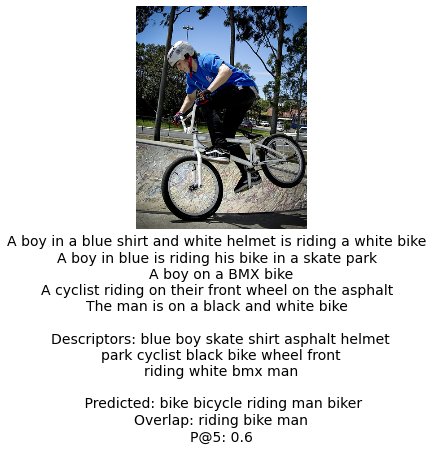
\includegraphics[scale=0.54]{chapters/TAL/bikeride}
\caption{\textit{Multiword image description example. Below the image
are the 5 captions describing the image, the union of words
that we take as targets, the top 5 predicted and the list of
correct words and the P@5 score for the given test case.}}
\label{fig:multiword-descriptors}
\end{figure}


\subsubsection{Single-concept image descriptions}
Even though we use separate portions of F8k and F30k for training and
testing, these subsets are still very similar. To test how general the
\textsc{Visual} word representations are, we use images from the ILSVRC2012
subset of ImageNet \citep{russakovsky2015imagenet} as benchmark. The major difference between these
images and the ones from F8k and F30k datasets is that labels of the
images in ImageNet are synsets from WordNet, which identify a single
concept present in the image instead of providing a natural
descriptions of its full content. Providing a quantitative evaluation
in this case is not straightforward for two main reasons. First, the
vocabulary of our model is restricted and the synsets in the ImageNet
dataset are quite varied. Second, the synset labels can be very precise,
much more so than the descriptions provided in the captions that we use
as our training data.

To attempt to solve the vocabulary mismatch problem, we use synset hypernyms
from WordNet as substitute target descriptors. If none of the lemmas
in the target synset are in the vocabulary of the model, the lemmas in
the hypernym synset are taken as new targets, until we reach the root
of the taxonomy. However, we find that in a large number of cases these hypernyms
are unrealistically general given the image. Figure \ref{fig:synset-descriptors}
illustrates these issues.

\begin{figure}
\centering
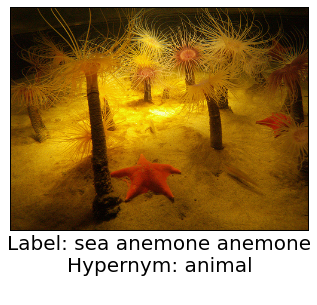
\includegraphics[scale=0.5]{chapters/TAL/starfish}
\caption{\textit{Example of the Single-concept image description task from
the validation portion of the ILSVRC2012 subset of ImageNet. The terms
"sea anemone" and "anemone" are unknown to \textsc{Visual} and "animal"
is the first word among it's hypernyms that appear in the vocabulary of F30k.}}
\label{fig:synset-descriptors}
\end{figure}
